\documentclass[12pt, a4paper]{article}
\usepackage{amsmath}
\usepackage{amsfonts}
\usepackage{amsthm}
\usepackage{mathtools}
\newtheorem{theorem}{Theorem}[section]
\newtheorem{definition}{Definition}[section]
\numberwithin{equation}{section}
\usepackage{pgfplots}
\pgfplotsset{width=10cm,compat=1.9}
\graphicspath{ {img/} }
\DeclareGraphicsExtensions{.png, .jpg}

\title{Likelihood}
\author{Kristian Wichmann}

\begin{document}
\maketitle

\section{Statistical models}
A \textit{statistical model} $\mathcal{P}$ is a family of probability distributions on a measurable space $(\mathcal{X},\mathbb{E})$ indexed by parameters $\theta$ from a parameter space $\Theta$. We can sum this up as:
\begin{equation}
\mathcal{P}=\{\nu_\theta|\theta\in\Theta\}
\end{equation}

\subsection{Dominated statistical models}
We call such a model \textit{dominated} if there exists a $\sigma$-finite measure $\mu$ on $(\mathcal{X},\mathbb{E})$, such that all the distributions in the model has a density function $f_\theta$ with respect to $\mu$. Or equivalently, that all the distributions is absolutely continuous with respect to $\mu$:
\begin{equation}
\forall\nu\in\mathcal{P}: \nu\ll\mu
\end{equation}
The Radon-Nikodym derivative $\frac{d\nu}{d\mu}$ is then a density function for $\nu$ with respect to $\mu$. We call $\mu$ a \textit{dominating measure} for the model.

This may all sound a little hairy, but in practice, the dominating measure will almost always be the Lebesgue measure (for continuous distributions), the counting measure (for discrete distributions), or some combination of the two.

\section{The likelihood function}

\subsection{Definition}
Let $\mathcal{P}$ be a dominated statistical model. The \textit{likelihood} function for an outcome $x\in\mathcal{X}$ is a function $L_x:\Theta\rightarrow\mathbb{R}$ associates a number to every parameter configuration:
\begin{equation}
L_x(\theta)=f_\theta(x)
\end{equation}
The interpretation of the likelihood function is, that the higher its value, the more likely it seems that $\theta$ is the true parameters of the model. Hence, we will often seek out the set of parameters which maximize the likelihood function. This process is known as \textit{maximum likelihood estimation} or MLE for short. Note that there's no mathematical justification of this process in itself.

\subsubsection{Example: Coin tosses}
We consider a repeated coin toss, each i.i.d. Bernoulli processes with parameter $p$ - the probability that the outcome is heads. If the coin is tossed $n$ times, the outcome space is $\mathcal{X}=\{0, 1, 2,\cdots, n\}$ where the number of the outcome heads is counted (the dominating measure is the counting measure). Given a specific outcome $k\in\mathcal{X}$, the likelihood function can be found by the binomial distribution:
\begin{equation}
L_k(p)=\binom{n}{k}p^k(1-p)^{n-k}
\end{equation}
Here $p\in\Theta=[0,1]$. Figure \ref{fig:binomial_likelihood} shows examples of this function.

\begin{figure}
\centering
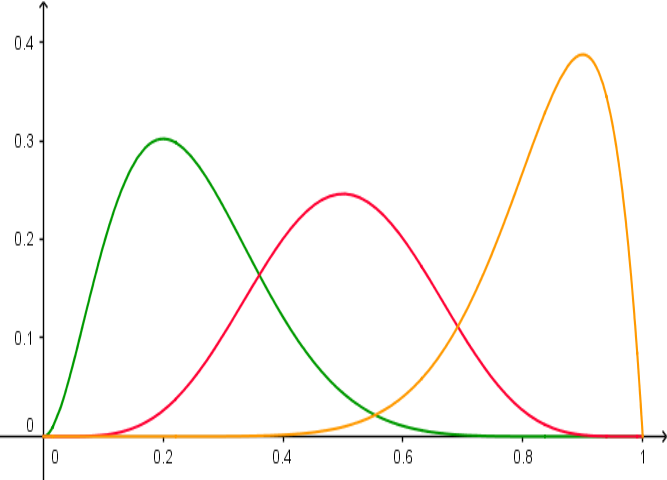
\includegraphics[width=.8\textwidth]{binomial_likelihood}
\caption{Likelihood function for $n=10$ and $k=2, 5, 9$ (green, red, orange) respectively.}
\label{fig:binomial_likelihood}
\end{figure}

Now, er can perform MLE by finding the value of the parameter $p$ which maximizes $L_k$. We differentiate using the product rule:
\begin{equation}
\frac{\partial L_k}{\partial p}=\binom{n}{k}\left(k(p^{k-1}(1-p)^{n-k}-p^k(n-k)(1-p)^{n-k-1}\right)
\end{equation}
For this to be zero, the binomial coefficient is irrelevant, so:
\begin{align}
k(p^{k-1}(1-p)^{n-k}&=p^k(n-k)(1-p)^{n-k-1}\Leftrightarrow \\
k(1-p)&=(n-k)p\Leftrightarrow \\
k&=np
\end{align}
In other words, $p_{\textrm{MLE}}=\frac{k}{n}$. This will probably not be much of a surprise to anyone.

However, this estimate might not always be sensible. Specifically, if you've made a very small amount of count throws. If $n=1$, you will conclude that $p=0$ or $p=1$, which meshes badly with our intuition about coin throws. This may be modelled as a \textit{prior distribution} of $p$, leading to a Bayesian analysis. Contrast with the case where $m\gg 1$: When we have a lot of repetitions, we will be more certain of the value of the parameter $p$. This idea of probability as a limit for a large number of repetitions is at the heart of the frequentist interpretation.

\subsection{The log-likelihood function}
When the density functions are nowhere zero, it often makes sense to deal with the logarithm of the likelihood function instead. Since the logarithm is a strictly monotonic function, this makes no difference for the purpose of MLE. Some presentations (this included), introduces a sign change as well:
\begin{equation}
l_x(\theta)=-\log f_\theta(x)
\end{equation}
So MLE means one of the following, equivalent procedures:
\begin{itemize}
\item Maximizing the likelihood function $L_x$.
\item Minimizing the log-likelihood function $l_x$.
\end{itemize}

\subsubsection{Example: Fish weights}
$n$ adult fish of the same species are caught and weighed. The weights can be reasonably modelled by a normal distribution $N(\mu,\sigma^2)$ (and so the dominating measure is the Lebesgue measure). For simplicity, we will assume that the variance is known from historical data. The observations are:
\begin{equation}
x=(w_1,w_2,\cdots,w_n)
\end{equation}
Now, the likelihood function is:
\begin{equation}
L_x(\mu)=\prod_{i=1}^n\frac{1}{\sqrt{2\pi\sigma^2}}\exp\left[-\frac{(w_i-\mu)^2}{2\sigma^2}\right]
\end{equation}
Here we see the practicality of taking the logarithm to get the log-likelihood: It turns a product like this into a much more manageable sum:
\begin{equation}
l_x(\mu)=-\log L_x(\mu)=-n\log\frac{1}{\sqrt{2\pi\sigma^2}}+\sum_{i=1}^n\frac{(w_i-\mu)^2}{2\sigma^2}
\end{equation}
Differentiating to find the minimum:
\begin{equation}
\frac{\partial l_x}{\partial\mu}=\frac{1}{2\sigma^2}\sum_{i=1}^n 2(w_i-\mu)=\frac{1}{\sigma^2}\sum_{i=1}^n w_i-n\mu
\end{equation}
Setting this to zero we find:
\begin{equation}
\mu_{\textrm{MLE}}=\frac{1}{n}\sum_{i=1}^n w_i
\end{equation}
Once again, hardy a surprising result.

\section{Score function and observed information function}
When the parameter space is an open subset of $\mathbb{R}^k$ (usually the case), we define these as follows:
\begin{itemize}
\item The \textit{score function} is the gradient of the log-likelihood:
\begin{equation}
V_x(\theta)=\nabla_\theta l_x(\theta)
\end{equation}
\item The \textit{observed information function} is the Hessian matrix of the log-likelihood function:
\begin{equation}
\mathcal{J}_x(\theta)=H_\theta[l_x(\theta)]=\nabla_\theta\nabla^t_\theta l_x(\theta)
\end{equation}
\end{itemize}



\subsection{Example: Coin toss}
As we saw above, here the likelihood is given by the binomial distribution:
\begin{equation}
L_k(p)=\binom{n}{k}p^k(1-p)^{n-k}\Rightarrow l_k(p)=-\log\binom{n}{k}-k\log p-(n-k)\log(1-p)
\end{equation}
Now to get the score function, we differentiate with respect to $p$:
\begin{equation}
V_k(p)=\frac{\partial l_x}{\partial p}=-\frac{k}{p}+\frac{n-k}{1-p}=\frac{(n-k)p-k(1-p)}{p(1-p)}=\frac{n-k}{p(1-p)}
\end{equation}
Three examples of the score function are shown in figure \ref{fig:binomial_score}.

\begin{figure}
\centering
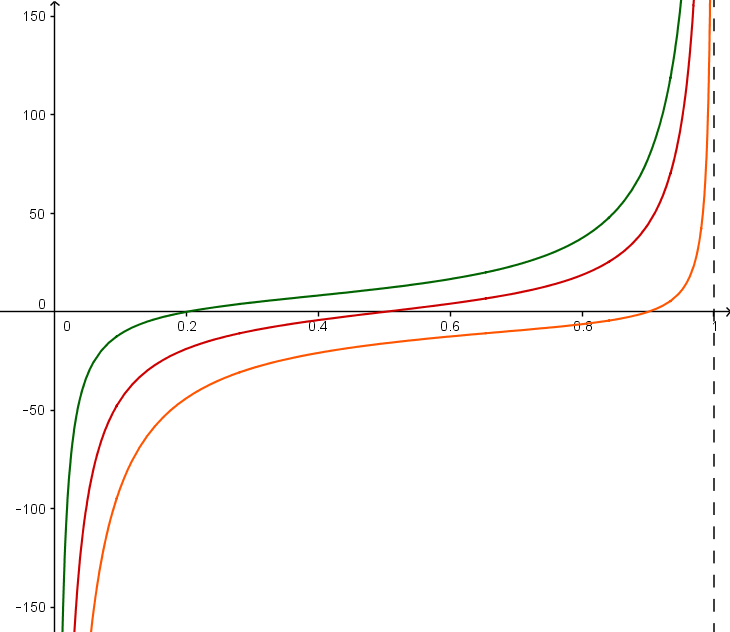
\includegraphics[width=.8\textwidth]{binomial_score}
\caption{Score function for $n=10$ and $k=2, 5, 9$ (green, red, orange) respectively.}
\label{fig:binomial_score}
\end{figure}

The observed information function, like the score function, is simply a scalar in this case:
\begin{equation}
\label{binomial_observed_information}
\mathcal{J}_k(p)=\frac{\partial V_k}{\partial p}=\frac{k}{p^2}+\frac{n-k}{(1-p)^2}
\end{equation}
Examples of these functions are shown in figure \ref{fig:binomial_observed_information}.

\begin{figure}
\centering
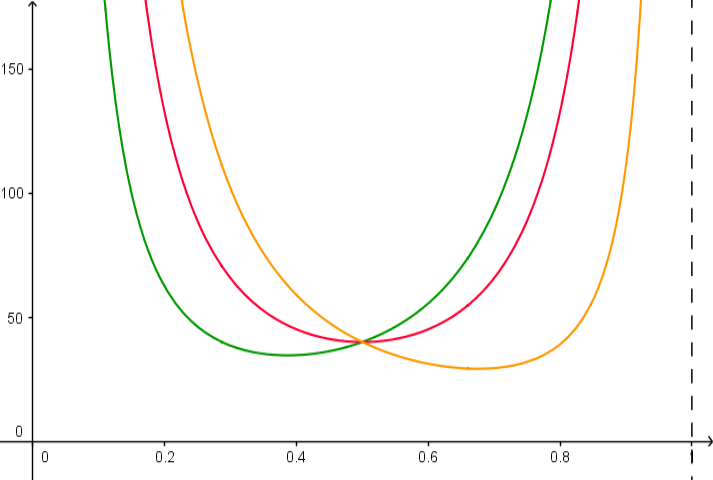
\includegraphics[width=.8\textwidth]{binomial_observed_information}
\caption{Observed information function for $n=10$ and $k=2, 5, 9$ (green, red, orange) respectively.}
\label{fig:binomial_observed_information}
\end{figure}


\section{Fisher information}
The \textit{Fisher information} (somtimes simply called the information) is the expected value of the observed information function:
\begin{equation}
\mathcal{I}(\theta)=E[\mathcal{J}_x(\theta)]
\end{equation}
Note that this is not a function of the actual outcome - The Fisher information is a property of the model, not the actual observations.

\subsection{Example: Bernoulli distribution}
The (log)likelihood for a random Bernoulli variable $X$ is:
\begin{equation}
L_x(p)=p^x(1-p)^{1-x}\Rightarrow l_x(p)=-x\log p-(1-x)\log(1-p)
\end{equation}
The score function is:
\begin{equation}
V_x(p)=-\frac{x}{p}+\frac{1-x}{1-p}
\end{equation}
The observed information function is:
\begin{equation}
\mathcal{J}_x(p)=\frac{x}{p^2}+\frac{1-x}{(1-p)^2}
\end{equation}
Now, to get the Fisher information we find the expectation value by summing over the two possible values of $x$:
\begin{align}
\mathcal{I}(p)=E[\mathcal{J}_x(p)]=&\sum_x P(X=x)\mathcal{J}_x(p)=p\frac{1}{p^2}+(1-p)\frac{1}{(1-p)^2}= \\
&\frac{1}{p}+\frac{1}{1-p}=\frac{1-p+p}{p(1-p)}=\frac{1}{p(1-p)}
\end{align}
This is simply the reciprocal of the variance of $X$.

\subsection{Example: Binomial distribution}
From equation \ref{binomial_observed_information} we know that:
\begin{equation}
\mathcal{J}_k(p)=\frac{k}{p^2}+\frac{n-k}{(1-p)^2}=\frac{(1-p)^2 k+p^2(n-k)}{p^2(1-p)^2}
\end{equation}
The numerator is:
\begin{equation}
(1-2p+p^2)k+p(n-k)=k-2pk+p^2 k+pn-pk=k-2pk+np^2
\end{equation}
So:
\begin{equation}
\mathcal{J}_k(p)=\frac{(1-2p)k+np^2}{p^2(1-p)^2}
\end{equation}
Now, the Fisher information is found by taking the expectation value of this, again by summing over outcomes (here $n+1$ possibilities). This means that everything that does not involve $k$ can be taken outside of the expectation:
\begin{equation}
\mathcal{I}(p)=E[\mathcal{J}_x(p)]=\frac{1}{p^2(1-p)^2}((1-2p)\ E[k]+np^2)
\end{equation}
The expected value of $k$ is $np$, so the parenthesis is equal to:
\begin{equation}
(1-2p)np+np^2=np-2np^2+np^2=np-np^2=n(p-p^2)=np(1-p)
\end{equation}
All in all, we get:
\begin{equation}
\mathcal{I}(p)=\frac{n}{p(1-p)}
\end{equation}


\end{document}